\documentclass[a4paper, 11pt]{article}
\usepackage[utf8]{inputenc}
\inputencoding{utf8}
\usepackage[english]{babel}
\usepackage{cite}
\usepackage{gensymb}
\usepackage{graphicx}
\graphicspath{ {images/} }
\usepackage[boxed]{algorithm2e}
\usepackage{amsmath}
\usepackage{relsize}

% Lengths and indenting
\setlength{\textwidth}{16.5cm}
\setlength{\marginparwidth}{1.5cm}
\setlength{\parindent}{0cm}
\setlength{\parskip}{0.15cm}
\setlength{\textheight}{25cm}
\setlength{\oddsidemargin}{0cm}
\setlength{\evensidemargin}{\oddsidemargin}
\setlength{\topmargin}{0cm}
\setlength{\headheight}{0cm}
\setlength{\headsep}{0cm}

\usepackage{hyperref} 
\usepackage[square,numbers]{natbib}
\bibliographystyle{abbrvnat}

\usepackage{cleveref}
\usepackage{tabularx}
\usepackage{float}

\newcommand*{\nolink}[1]{%
	\begin{NoHyper}#1\end{NoHyper}%
}

%opening
\title{Bachelor practical: Report}
\author{Marco Unternährer}
\date{\today}

\begin{document}
\maketitle

\section{Introduction}

Training a spiking neural network is a challenging task.
Neuromorphic vision researchers have to create spiking datasets since there is a lack of such datasets publicly available .
One method for converting static image datasets into neuromorphic vision datasets was proposed by moving a sensor in front of an image \cite{Orchard2015}.

Another approach for training a spiking neural network was developed by researchers at the Institute of Neuroinformatics \cite{Diehl2015}.
A non-spiking neural network is trained by using a regular static image dataset like MNIST or Caltech-101.
The resulting weights of the trained neural network can then be used to create a spiking neural network.
One constraint for this to work is that units must have zero bias.\\

The task for this bachelor practical was to train a convolutional neural network on the Caltech-101 dataset.



\section{Image Classification on Caltech-101}
This section will give a short introduction to the Caltech-101 dataset, the used methods and techniques.

\subsection{Caltech-101} \label{sec:caltech101}
Caltech-101 is a dataset of pictures of objects, which was collected in September 2003 by \citet{Fei-Fei2007} at the California Institute of Technology.
Most categories have about 50 images, but the number ranges from 40 to 800 per category \cite{Fei-Fei2007}.
Caltech-101 contains a total of 9'146 images, split between 101 distinct object categories (faces, watches, ants, pianos, etc.) and a background category \cite{Caltech101Wiki}.
The size of each image is roughly 300 x 200 pixels \cite{Fei-Fei2007}.

Unlike other datasets, Caltech-101 doesn't have a predefined split between train and test images.
\citet{Fei-Fei2007} suggest to use a fixed number of images per category for training and testing.
Due to the fact that categories have vastly different number of images, the accuracy per category can also vary a lot.
On an additional note, \cite{Fei-Fei2007} pointed out that if a fixed number of images per category is chosen, then the overall error rate should be reported.
However, if all the available images are being used for testing, then the average error rate across categories should be reported.\\

The state-of-the-art classification on the Caltech-101 dataset has an accuracy of 91.44\% \cite{He2014}.


\subsection{Convolutional Neural Network}
A convolutional neural network (CNN) is a type of feed-forward artificial neural network.
CNNs are biologically-inspired variants of multilayer perceptrons \cite{DLCNN}.
From Hubel and Wiesel's early work on the cat's visual cortex \cite{Hubel1968}, it is known that the visual cortex contains a complex arrangement of cells \cite{DLCNN}.
These cells are sensitive to small sub-regions of the visual field, called a receptive field \cite{DLCNN}.
The sub-regions are tiled to cover the entire visual field.
These cells act as local filters over the input space and are well-suited to exploit the strong spatially local correlation present in natural images.
Additionally, two basic cell types have been identified: Simple cells respond maximally to specific edge-like patterns within their receptive field.
Complex cells have larger receptive fields and are locally invariant to the exact position of the pattern \cite{DLCNN}.

Like their biological relatives, units in a CNN take advantage of the 2D structure of the input data (images or other 2D input such as a speech signal).
This is achieved with local connections and tied weights followed by some form of pooling which results in translation invariant features \cite{StanfordTutCNN2015}.


\subsection{Batch Normalization}
Stochastic gradient descent (SGD) and its variants are proven to be an effective way of training deep networks \cite{Ioffe2015}.
However, they require careful tuning of the model-hyperparameters, specifically the learning rate used in optimization, as well as the initial values for the model parameters \cite{Ioffe2015}.
Inputs to each layer are affected by parameters of all preceding layers, which makes training highly complicated \cite{Ioffe2015}.
Thus, the smallest changes to the network amplify as the network becomes deeper \cite{Ioffe2015}.
The problem seems to be the change in the distribution of layer's inputs, because the layers need to continuously adapt to the new distribution \cite{Ioffe2015}.
When the input distribution to a learning system changes, it is said to experience covariate shift \cite{Shimodaira2000}.

Batch normalization is a new mechanism that takes a step towards reducing internal covariate shift, and in doing so dramatically accelerates the training of deep neural nets \cite{Ioffe2015}.
It accomplishes this via a normalization step that fixes the means and variances of layer inputs \cite{Ioffe2015}.
Simplifications of the idea have to be made in order to accommodate mini-batches in stochastic gradient training: each mini-batch produces estimates of the mean and variance of each activation.
For completeness, the batch normalization transform algorithm by \citet{Ioffe2015} can be seen in \autoref{alg:bn}.

For convolutional layers, the normalization also has to obey the convolutional property – so that different elements of the same feature map, at different locations, are normalized in the same way \cite{Ioffe2015}.
To achieve this, we jointly normalize all the activations in a mini-batch, over all locations \cite{Ioffe2015}.

\begin{algorithm}[H]
	\DontPrintSemicolon
	\SetKwInOut{Input}{Input}\SetKwInOut{Output}{Output}
	\Input{Values of x over a mini-batch: $B = \{x_{1..m}\}$; \newline Parameters to be learned: $\gamma, \beta$}
	\Output{\{$y_i = BN_{\gamma,\beta}(x_i)$\}}
	\BlankLine
	\begin{algomathdisplay}
		\begin{aligned}
		\mu_B &\leftarrow \frac{1}{m} {\sum}_{i=1}^{m} x_i & \text{// mini-batch mean}&\\
		\sigma_B^2 &\leftarrow \frac{1}{m} {\sum}_{i=1}^{m} (x_i - \mu_B)^2 & \text{// mini-batch variance}&\\
		\hat{x_i} &\leftarrow \frac{x_i - \mu_B}{\sqrt{\sigma_B^2 + \epsilon}} & \text{// normalize}&\\
		y_i &\leftarrow \gamma \hat{x_i} + \beta \equiv BN_{\gamma,\beta}(x_i) & \text{// scale and shift}&\\
		\end{aligned}
	\end{algomathdisplay}

	\caption{Batch Normalizing Transform, applied to activation x over a mini-batch}
	\label{alg:bn}
\end{algorithm}



\subsection{Cyclical Learning Rates}
\citet*{Bengio2012} says that the learning rate is the most important hyper-parameter to optimize and if "there is only time to optimize one hyper-parameter and one uses stochastic gradient descent, then this is the hyper-parameter that is worth tuning".
It is well known that too small a learning rate will make a training algorithm converge slowly while too large a learning rate will make the training algorithm diverge \cite{Zeiler2012}.
Hence one must experiment with a variety of learning rates and schedules (i.e., the timing of learning rate changes) \cite{Smith2015}.

The conventional wisdom is that the learning rate should be a single value that monotonically decreases during the training \cite{Smith2015}.
However, \nolink{\citeauthor{Smith2015}} demonstrates the surprising phenomenon that increasing the learning rate is overall beneficial and thus proposes to let the global learning rate vary cyclically within a band of values rather than setting it to a fixed value \cite{Smith2015}.



\section{Experimental Setup}

\subsection{Data Pre-processing \& Data Augmentation}
Since the heights and widths of the Caltech-101 images vary, all images were scaled to a common size. 
Like \citet{Orchard2015}, each image was resized to be as large as possible while maintaining the original aspect ratio and ensuring that width does not exceed 240 pixels and height does not exceed 180 pixels.

After running a few experiments with a fairly deep architecture, it became clear, that the roughly 9k images of the Caltech-101 dataset were not enough to accomplish a decent test accuracy.
Starting from the original dataset, data augmentation was pursued by randomly transform each picture ten times, and thus leading to approximately 100k images (including the original dataset).

Using an image data generator \cite{keras}, we ended up with the following augmentation parameters:
\begin{itemize}
	\item rotation: random with angles in the range 0$\degree$ to 20$\degree$
	\item translation: random with shift between 0\% and 20\% of total width/height
	\item flipping: horizontal/vertical, yes or no (Bernoulli)
	\item zooming: random zoom axis by +/- 20\%
\end{itemize}

The created images were then resized again, but with the difference that the images were padded with the edge pixels to fill the needed aspect ratio.
The pixel values were normalized to the range of (0, 1) after loading the images.
Data standardization, subtracting the mean and dividing by the standard deviation, was also applied.\\

The generated images are available online and can be downloaded under \cite{UnternaehrerGenImg}.


\subsection{Architecture}
Our architectures were inspired by \citet{Simonyan2015} and \citet{CS231nCNN}.
However, due to the fact that the neural network will be converted into a spiking neural network, we had two constraints.
The first constraint was that units must not have any bias.
The second constraint had to do with performance: Since the network should be able to classify pictures near real-time, we limited the depth of our architecture to three convolutional and two fully connected layers.
Obviously, when introducing batch normalization, there are more layers.
Those additional layers should not have a high impact on the speed of classification though, since batch normalization is only a linear transformation.

\Cref{tab:base-arch,tab:bn-arch,tab:no-bn-arch} show the used network architectures.

\begin{table}[H]
	\begin{center}
		\begin{tabularx}{.5\linewidth}{|X|l|}
			\hline \textbf{Layer type} & \textbf{Parameters} \\ 
			\hline convolution & 128x5x5, stride 2x2 \\ 
			\hline relu &\\
			\hline maxpool &  2x2\\ 
			\hline convolution & 256x3x3 \\ 
			\hline relu &\\
			\hline maxpool &  2x2\\ 
			\hline convolution & 512x3x3 \\ 
			\hline relu &\\
			\hline maxpool &  2x2\\ 
			\hline full &  1024 \\ 
			\hline relu &\\
			\hline full &  102 \\
			\hline softmax & \\
			\hline
		\end{tabularx}
	\end{center}
	\caption{Base Network Architecture}
	\label{tab:base-arch}
\end{table}


\begin{table}[H]
	\begin{center}
		\begin{tabularx}{.5\linewidth}{|X|l|}
			\hline \textbf{Layer type} & \textbf{Parameters} \\ 
			\hline convolution & 128x5x5, stride 2x2 \\ 
			\hline batch normalization & \\
			\hline relu &\\
			\hline maxpool &  2x2\\ 
			\hline convolution & 256x3x3 \\ 
			\hline batch normalization & \\
			\hline relu &\\
			\hline maxpool &  2x2\\ 
			\hline convolution & 512x3x3 \\ 
			\hline batch normalization & \\
			\hline relu &\\
			\hline maxpool &  2x2\\ 
			\hline full &  1024 \\ 
			\hline relu &\\
			\hline full &  102 \\
			\hline softmax & \\
			\hline
		\end{tabularx}
	\end{center}
	\caption{Network Architecture with Batch Normalization}
	\label{tab:bn-arch}
\end{table}

\begin{table}[H]
	\begin{center}
		\begin{tabularx}{.5\linewidth}{|X|l|}
			\hline \textbf{Layer type} & \textbf{Parameters} \\ 
			\hline convolution & 128x5x5, stride 2x2 \\ 
			\hline relu &\\
			\hline maxpool &  2x2\\ 
			\hline dropout & 0.35 \\
			\hline convolution & 256x3x3 \\ 
			\hline relu &\\
			\hline maxpool &  2x2\\ 
			\hline dropout & 0.35 \\
			\hline convolution & 512x3x3 \\ 
			\hline relu &\\
			\hline maxpool &  2x2\\ 
			\hline dropout & 0.35 \\
			\hline full &  1024 \\ 
			\hline relu &\\
			\hline dropout & 0.5 \\
			\hline full &  102 \\
			\hline softmax & \\
			\hline
		\end{tabularx}
	\end{center}
	\caption{Network Architecture without Batch Normalization}
	\label{tab:no-bn-arch}
\end{table}



\subsection{Training}
The splitting of the generated images into training and test samples was stratified, meaning that each class had 90\% in the training set and 10\% in the test set.
That training set was then further split into 10 folds, such that cross-validation could be applied later on.

Stochastic gradient descent was used as the optimizer, with Nesterov momentum of 0.9 and a learning rate decay of 5e-4.
Batch size was 64 most of the time, but was decreased for some architecture configurations due to GPU memory overallocation.

We applied a triangular learning rate schedule in order to speed up training as well as reduce the need for hyper-parameter optimization \cite{Smith2015}.
In combination with a batch normalized network, the minimum learning rate was 0.001, the maximum learning rate was 0.02 and the step size was set to 8 times the number of iterations in an epoch.


\subsection{Implementation Details}
The neural network framework of choice was Keras \cite{keras}.
Keras is a minimalist, highly modular neural networks library, written in Python and running on top of Theano.
Being Python-based and especially developed with a focus on enabling fast experimentation, it was a good candidate for this project.
Most importantly, Keras seemed to provide almost all needed functionality out of the box.
Another relevant aspect, that lead to the decision to use Keras, was that model architectures are created with code.
That made rapid prototyping and experimentation feasible.\\

The networks were trained on a system equipped with a single NVIDIA GTX 970 GPU.\\

The source code for the entire bachelor practical can be found at \cite{UnternaehrerCode}.

\section{Results}
After running many preliminary experiments, we have settled for the architectures shown in \cref{tab:bn-arch} (with batch normalization) and \cref{tab:no-bn-arch} (without batch normalization).

Unfortunately, the high imbalance of the dataset was not considered in the preliminary experiments and \cref{app:imbalance} explains the mistakes made.

Apart from creating a good classifier for the Caltech-101 dataset, we had specific experiments to run in mind, which we describe in \cref{sec:batch,sec:data,sec:kernel,sec:lr}.
\Cref{sec:cv} shows the cross-validation of the best performing network, which also respects the needed constraints.



\begin{table}[!h]
	\begin{center}
		\begin{tabularx}{\linewidth}{|X|l|l|}
			\hline \textbf{Experiment} & \textbf{Validation Acc} & \textbf{Test Acc}\\ 
			\hline base line - batch normalization, with zero bias constraint, \cref{fig:bn_bias} & 82.66\% & 82.41\% \\
			\hline batch normalization, without zero bias constraint, \cref{fig:bn_no-bias} & 82.92\% & 82.54\% \\
			\hline no batch normalization, with zero bias constraint, \cref{fig:no-bn_bias} & 73.04\% & 73.98\% \\
			\hline no batch normalization, without zero bias constraint, \cref{fig:no-bn_no-bias} & 78.09\% & 78.26\% \\
			\hline no data standardization, \cref{fig:bn_no-data-standardization} & 82.93\% & 81.86\% \\
			\hline increased kernel to 9x9 in first convolutional layer, \cref{fig:conv1-9x9} & 82.99\% & 82.23\% \\
			\hline triangular learning rate schedule, start with minimum lr, \cref{fig:triangular-min-to-max} & 77.91\% & 77.40\% \\
			\hline
		\end{tabularx}
	\end{center}
	\caption{Experiment Results}
	\label{tab:experiment-results}
\end{table}

\clearpage
\subsection{Batch Normalization and Zero Bias Constraint} \label{sec:batch}

As we can see in \cref{fig:bn_bias,fig:bn_no-bias}, there is basically no difference in loss or accuracy when introducing the zero bias constraint in the case we train with the batch normalization architecture (\cref{tab:bn-arch}).
However, comparing \cref{fig:no-bn_bias,fig:no-bn_no-bias} indicates that the zero bias constraint has quite an impact on training speed as well as the resulting validation and test accuracies (see \cref{tab:experiment-results}).


\begin{figure}[H]
	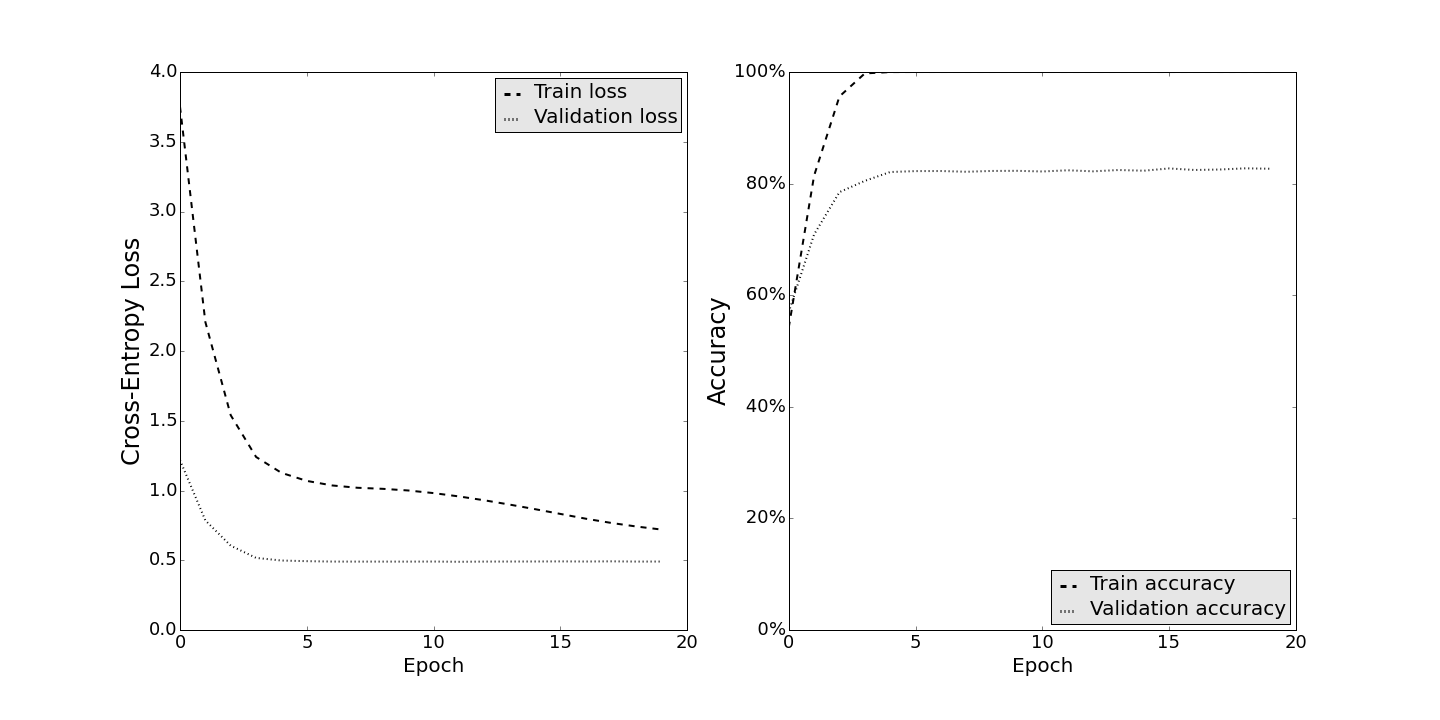
\includegraphics[width=\linewidth]{bn_bias-constraint.png}
	\caption{Base line - batch normalization, with zero bias constraint}
	\label{fig:bn_bias}
\end{figure}

\begin{figure}[H]
	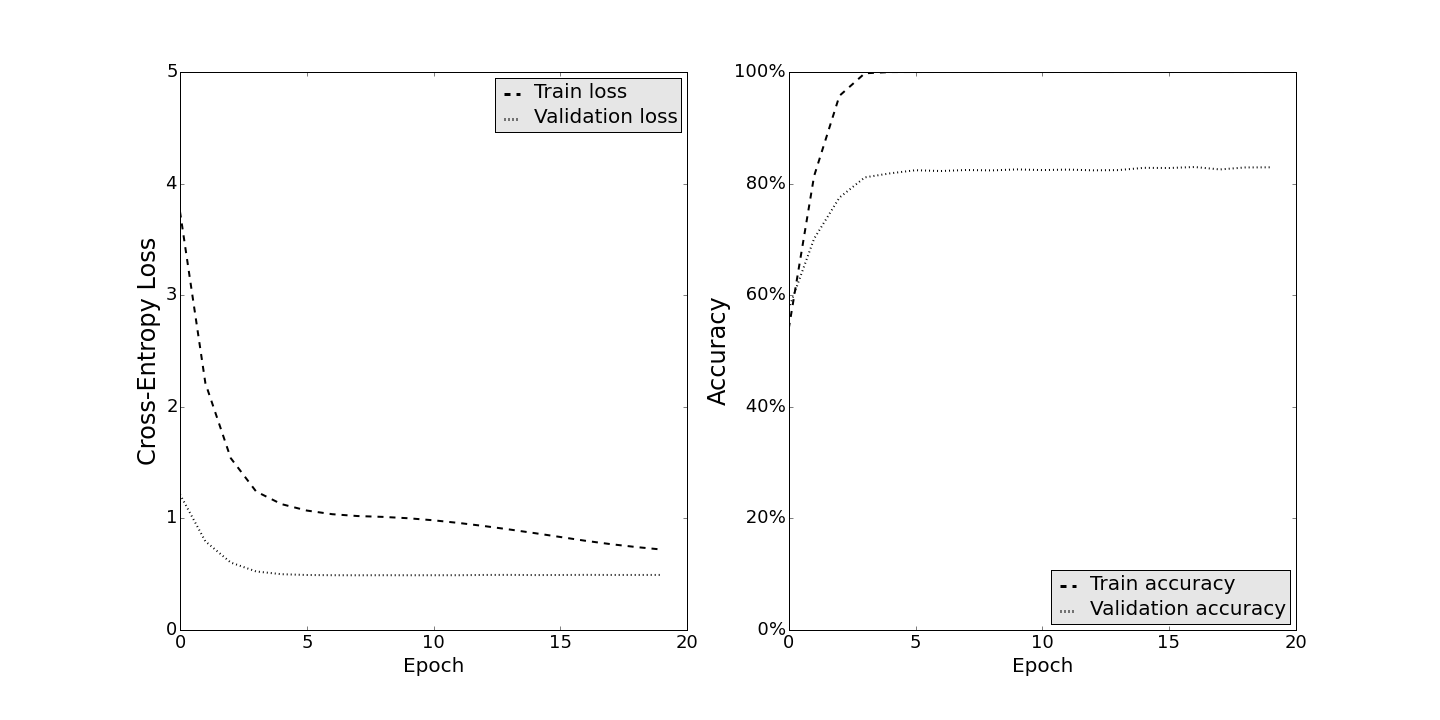
\includegraphics[width=\linewidth]{bn_no-bias-constraint.png}
	\caption{Batch normalization, without zero bias constraint}
	\label{fig:bn_no-bias}
\end{figure}

\begin{figure}[H]
	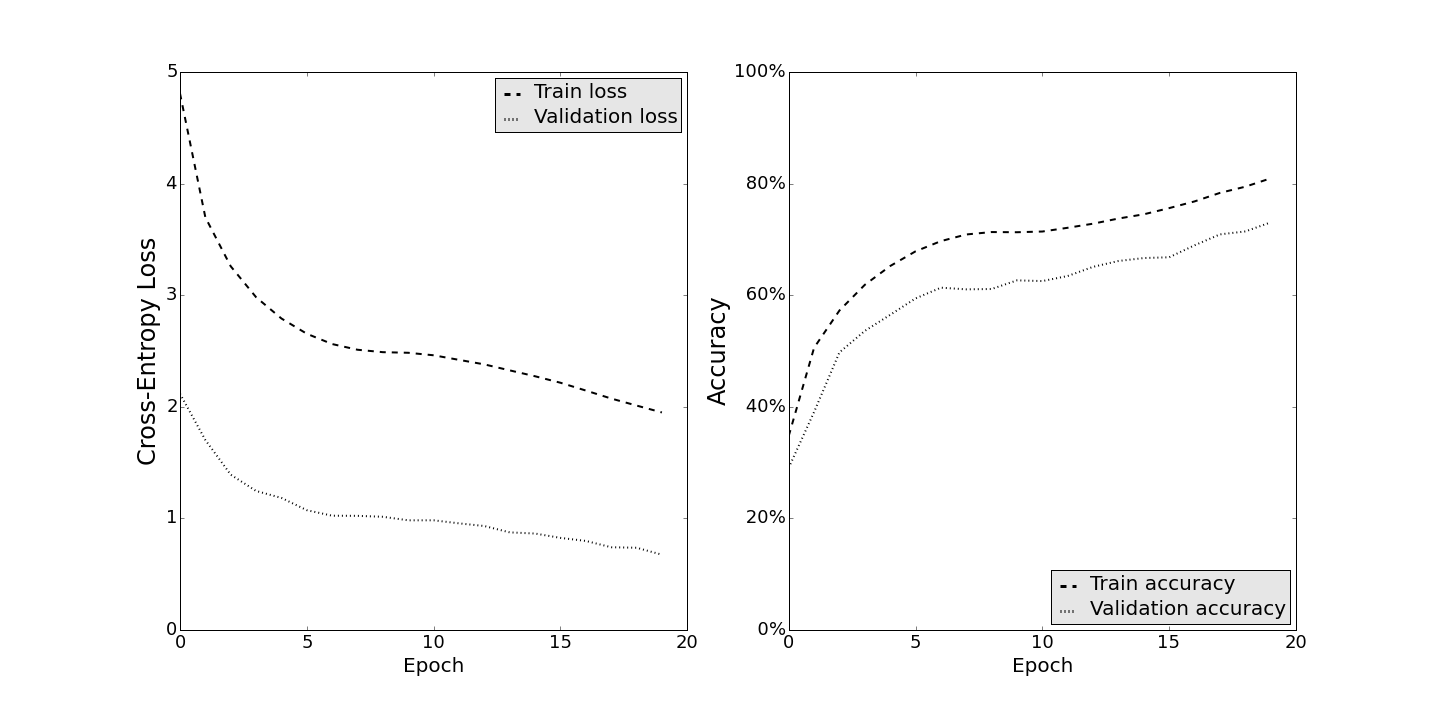
\includegraphics[width=\linewidth]{no-bn_bias-constraint.png}
	\caption{No batch normalization, with zero bias constraint}
	\label{fig:no-bn_bias}
\end{figure}

\begin{figure}[H]
	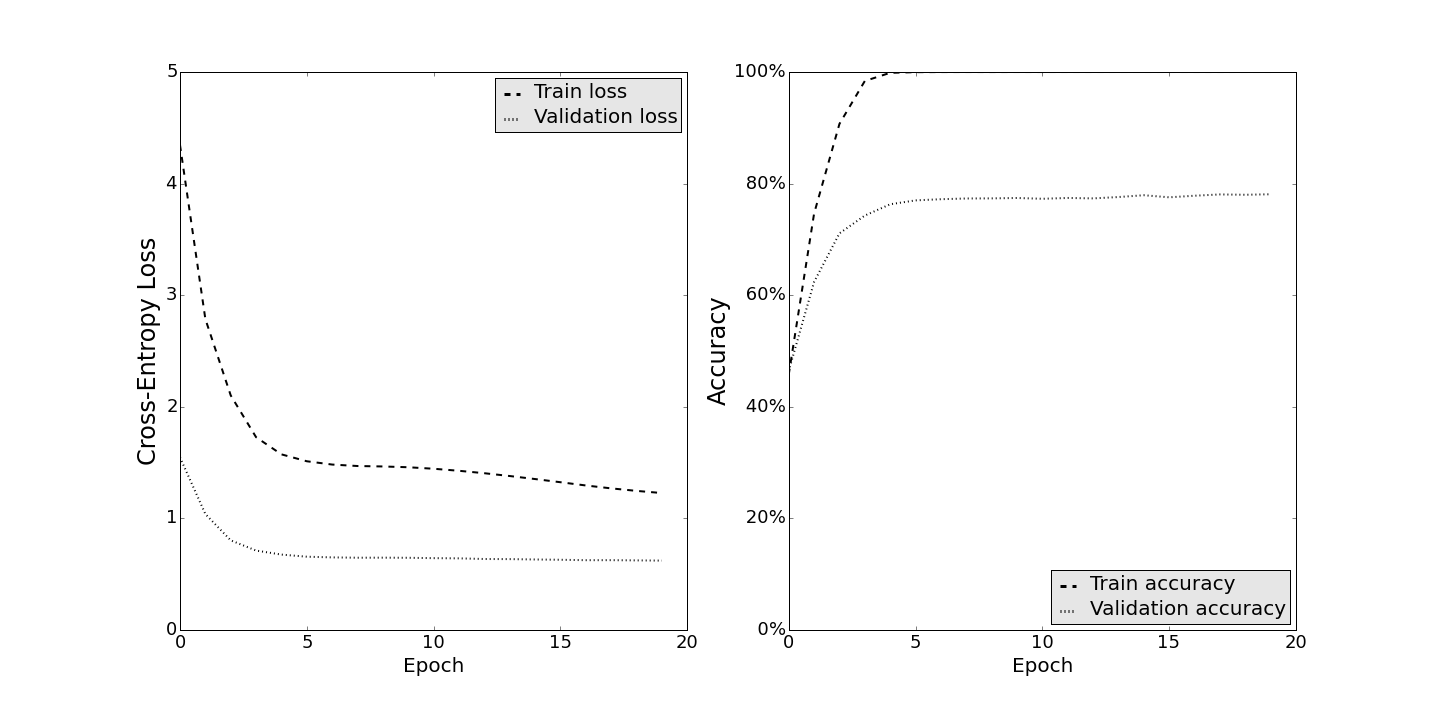
\includegraphics[width=\linewidth]{no-bn_no-bias-constraint.png}
	\caption{No batch normalization, without zero bias constraint}
	\label{fig:no-bn_no-bias}
\end{figure}

\clearpage

\subsection{Data Standardization} \label{sec:data}

We have trained the same network as the base line, but with the exception that no data standardization was applied.
Data normalization, bringing the pixel values into the range of (0, 1), however, was applied.
Comparing experiments \cref{fig:bn_bias,fig:bn_no-data-standardization} shows that there is virtually no difference in the behavior of the networks.
Also, from \cref{tab:experiment-results} it can be seen that the validation and test accuracies are within a very small range.
This suggests that using batch normalization also eliminates the need to previously standardize the data to have zero mean and unit standard deviation.

\begin{figure}[H]
	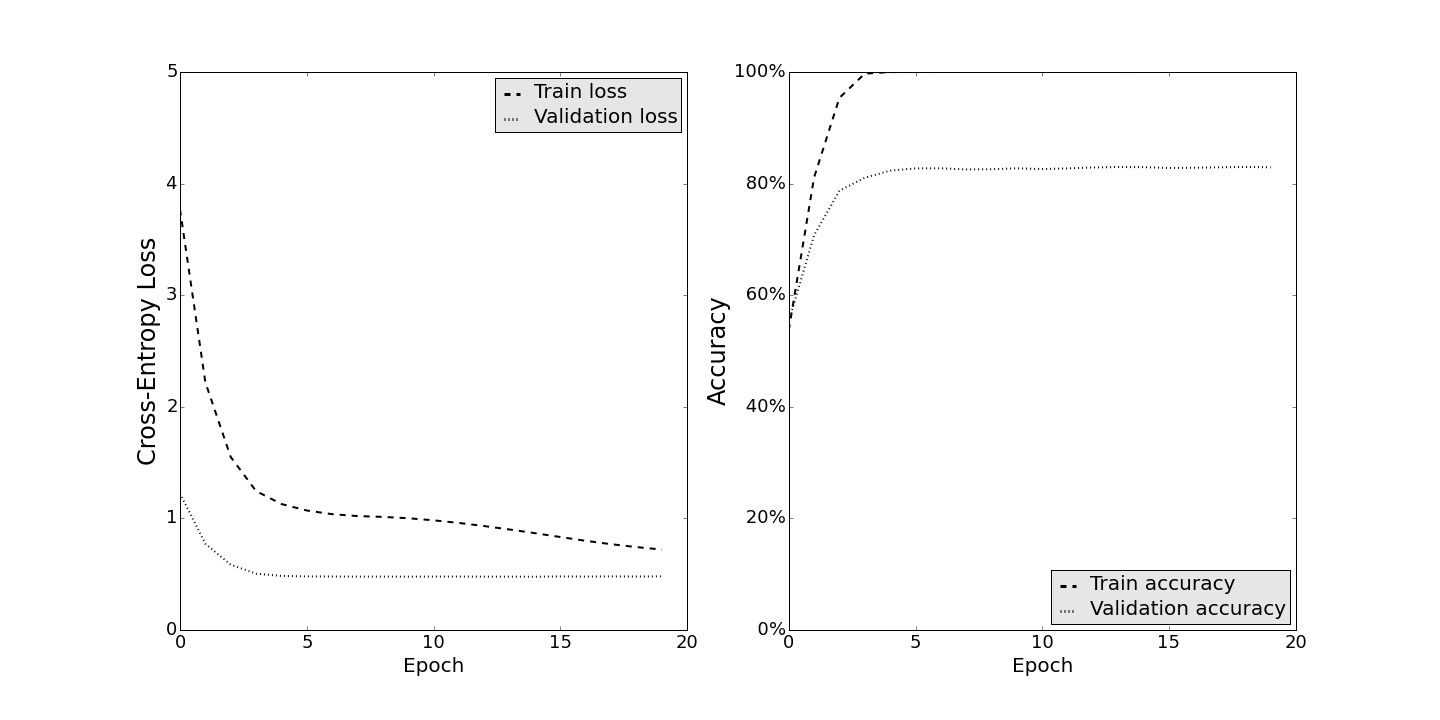
\includegraphics[width=\linewidth]{no-data-standardization.png}
	\caption{No data standardization }
	\label{fig:bn_no-data-standardization}
\end{figure}

\clearpage

\subsection{Convolutional Kernel Size} \label{sec:kernel}

In this experiment, we simply increased the kernel size in the first convolutional layer from 5x5 to 9x9. Comparing \cref{fig:bn_bias,fig:conv1-9x9} as well as the accomplished results in \cref{tab:experiment-results} indicates that the kernel size has no major impact on the performance.
\begin{figure}[H]
	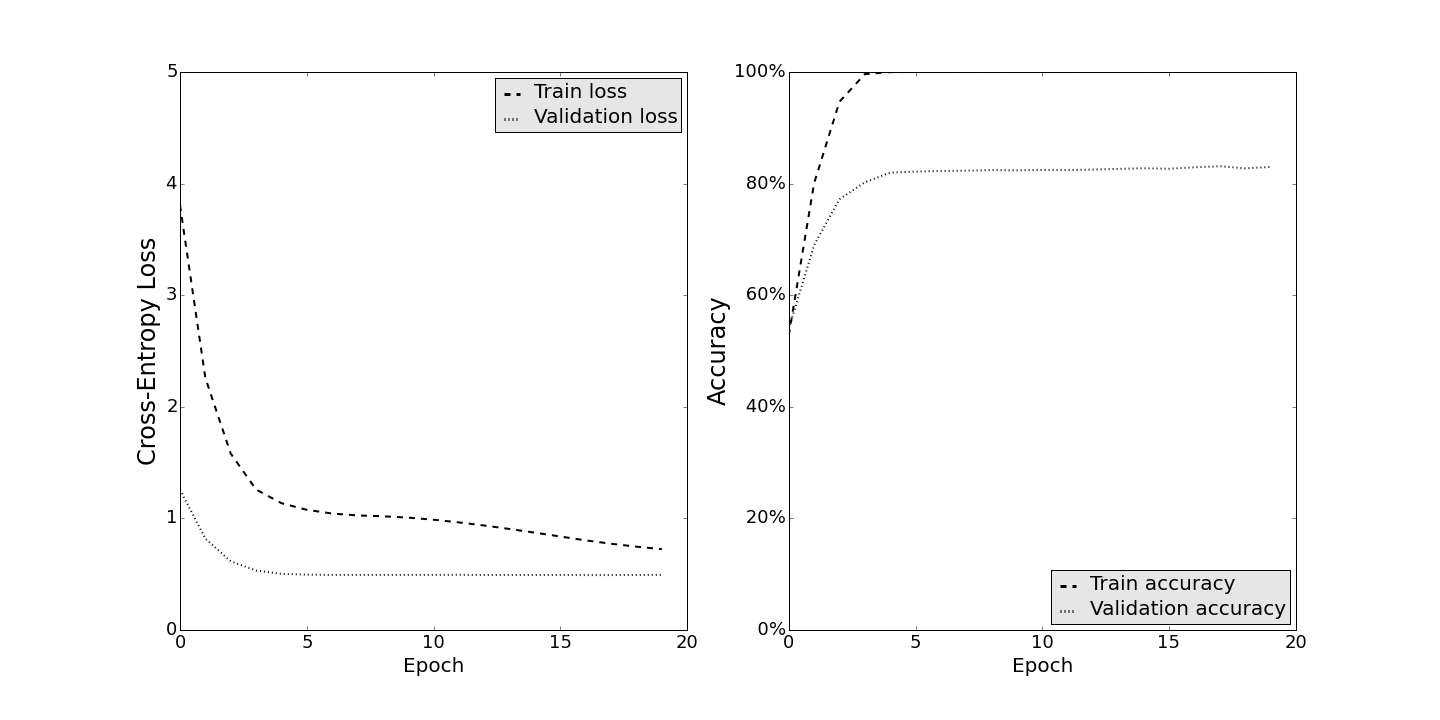
\includegraphics[width=\linewidth]{conv1-9x9.png}
	\caption{Increased kernel to 9x9 in first convolutional layer }
	\label{fig:conv1-9x9}
\end{figure}

\clearpage

\subsection{Triangular Learning Rate} \label{sec:lr}
\citet{Smith2015} suggests to start the triangular learning rate schedule with the minimum, then increasing to the maximum, and decreasing again.
However, one suggestion to accelerate batch normalized networks is to increase the learning rate decay \cite{Ioffe2015}.
Comparing \cref{fig:bn_bias,fig:triangular-min-to-max} and their according validation and test accuracies (\cref{tab:experiment-results}), this suggests that starting out with the maximum learning rate, then decreasing to the minimum is the preferred way when using a triangular learning rate schedule for a batch normalized network.

\begin{figure}[H]
	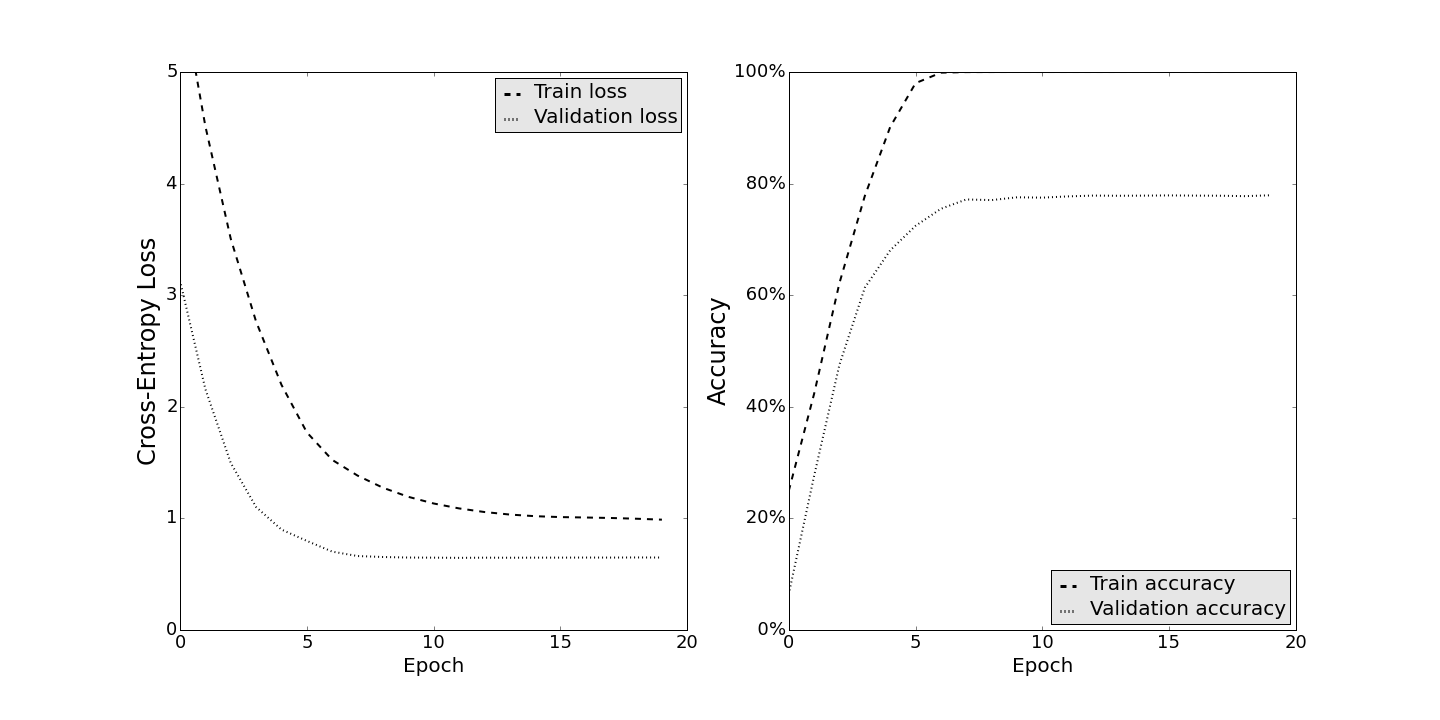
\includegraphics[width=\linewidth]{triangular-min-to-max.png}
	\caption{Triangular Learning Rate Schedule, start with minimum lr }
	\label{fig:triangular-min-to-max}
\end{figure}

\clearpage

\subsection{Cross-Validation} \label{sec:cv}

We ran the batch normalized network architecture (\cref{tab:bn-arch}) on a 10-fold cross-validation.
The resulting mean validation accuracy was 82.21\%, while the mean test accuracy was 82.10\%.

\begin{figure}[H]
	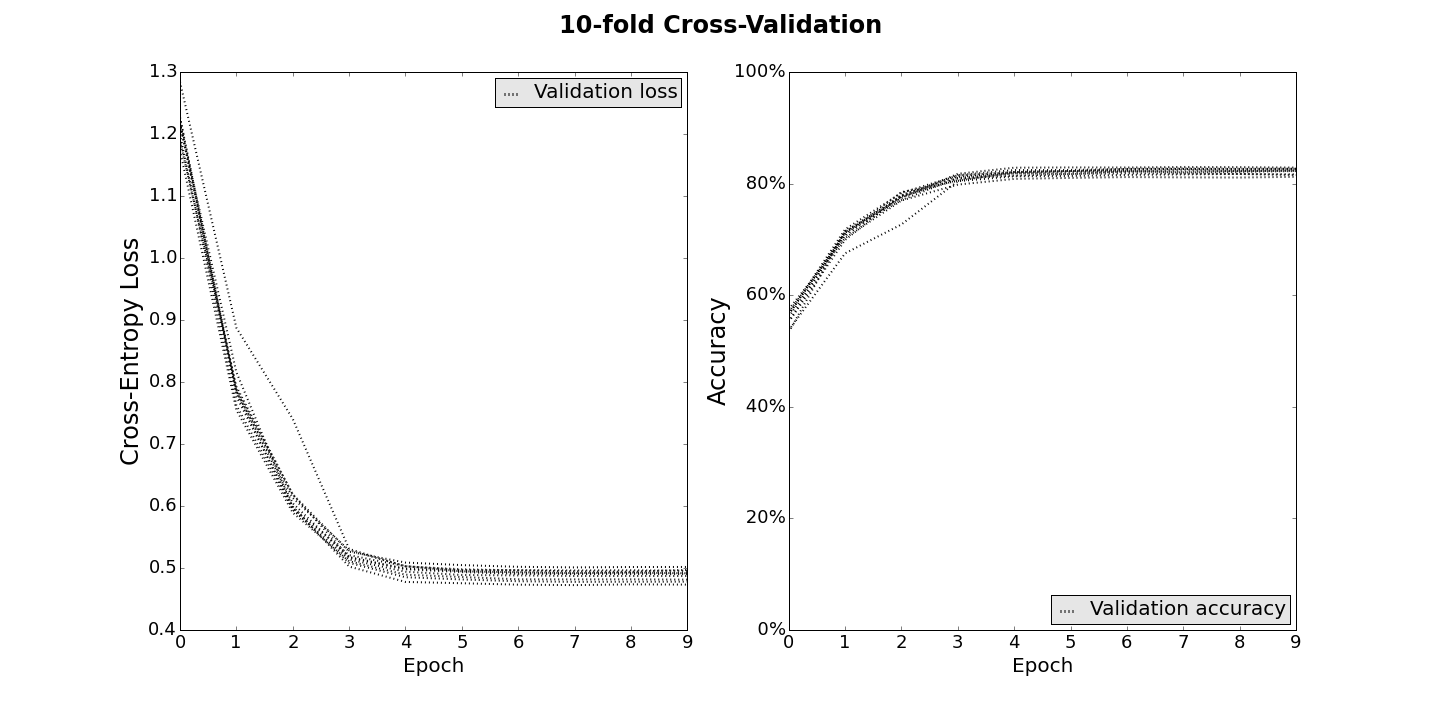
\includegraphics[width=\linewidth]{cross-val.png}
	\caption{Cross-Validation}
	\label{fig:cross-val}
\end{figure}


\section{Conclusion}
In order to achieve a decent accuracy on a fairly deep neural network, having enough data is important \cite{Domingos2014}.
If not enough data is available, as in our case, coming up with a way to generate more data is recommended \cite{Plankton2015}.

Creating sensible network architectures is not easy.
We relied on the expertise of several authors \cite{Simonyan2015,CS231nCNN}, which lead us to the base architecture described in \cref{tab:base-arch}.

Batch normalization can speed up training significantly \cite{Ioffe2015}.
In this work, we have shown that batch normalization is outperforming non-batch-normalized models, especially if we have a zero bias constraint.
Hence, we recommend to use batch normalization whenever the zero bias constraint is needed.\\


Future work should focus on the performance impact of an additional convolutional layer as well as a running more hyper-parameter optimization experiments.
These methods will hopefully lead to getting closer to the state-of-the-art accuracy for the Caltech-101 dataset of 91.44\% \cite{He2014}.


\clearpage
\bibliography{C:/Users/Marco/Documents/MendeleyBibtex/Bsc-Practical,websites}

\appendix
\section{Imbalanced Data} \label{app:imbalance}
As we have already mentioned in \cref{sec:caltech101}, the dataset is highly imbalanced.
Unfortunately, we have discovered only at a very late stage of this bachelor practical, that this imbalance was not considered in the numerous experiments we have already run.
Thus, all previous experiments were rendered invalid by this mistake.

We have developed a function, which calculates the accuracy on a per-category basis.
The mean of those accuracies were then used as the overall accuracy, as \citet{Fei-Fei2007} suggest in order to normalize the performance across categories.
Additionally, category weights were calculated and applied while training, such that the effects of the imbalance were less severe.


\subsection{Results}
Below we show some experiments, which could be of interest, even though the validation and test accuracies are not considering the imbalance of the categories and thus overconfident.

\subsubsection{Dropout}
Comparing the training and the validation accuracy in \cref{fig:app_dropout_base}, it seemed that the network is overfitting (architecture see \cref{tab:bn-arch}).
To circumvent this, we ran an experiment, where we introduced dropout (with probability 0.5) between the fully connected layer (see \cref{fig:app_dropout_exp}).
No significant increase in the validation and test accuracies was the result of this experiment (see \cref{tab:app_dropout_experiment-results}).
\begin{table}[!h]
	\begin{center}
		\begin{tabularx}{\linewidth}{|X|l|l|}
			\hline \textbf{Experiment} & \textbf{Validation Acc*} & \textbf{Test Acc*}\\ 
			\hline base line, \cref{fig:app_dropout_base} & 88.08\% & 88.20\% \\
			\hline dropout (0.5) between fully connected layers, \cref{fig:app_dropout_exp} & 88.44\% & 88.30\% \\
			\hline
		\end{tabularx}
	\end{center}
	\caption{Dropout experiment results - Not considering imbalance of categories}
	\label{tab:app_dropout_experiment-results}
\end{table}
\begin{figure}[H]
	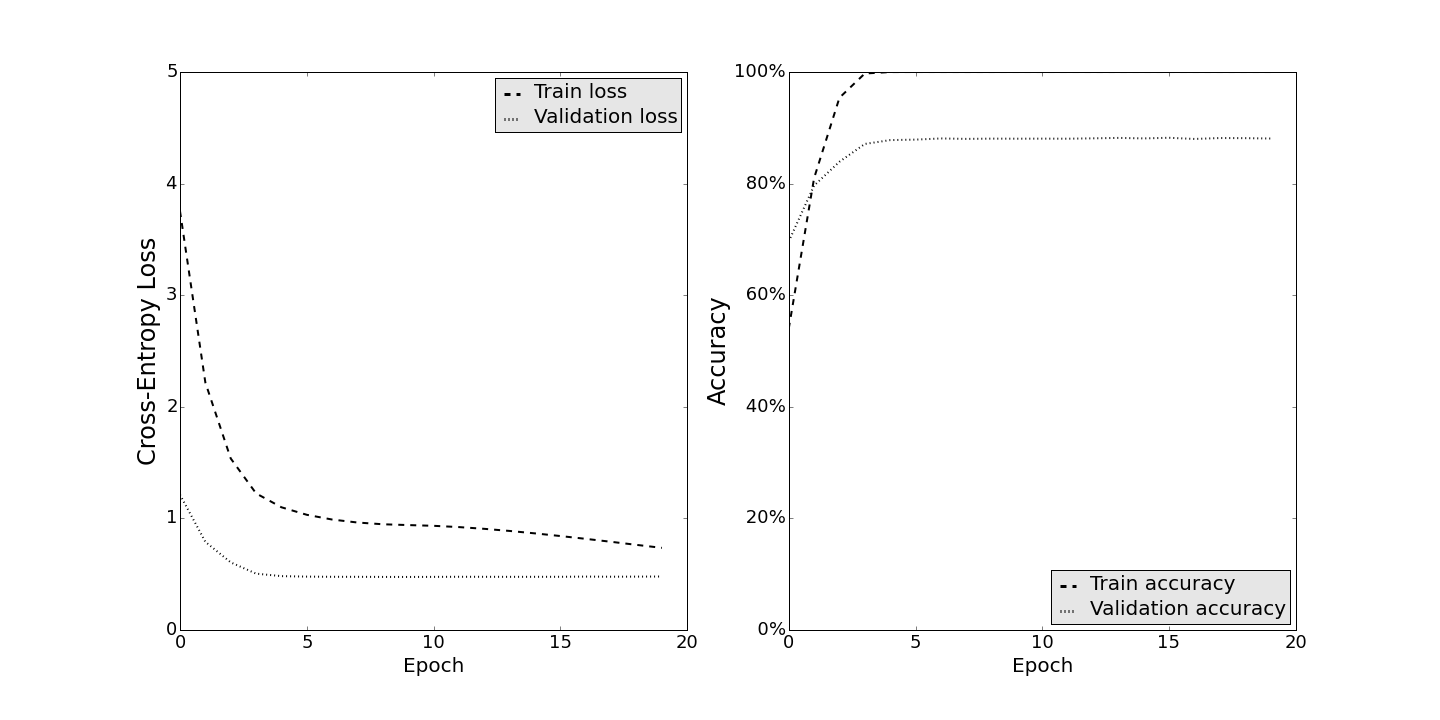
\includegraphics[width=\linewidth]{appendix-bn_triangular_e20.png}
	\caption{Base line for dropout}
	\label{fig:app_dropout_base}
\end{figure}

\begin{figure}[H]
	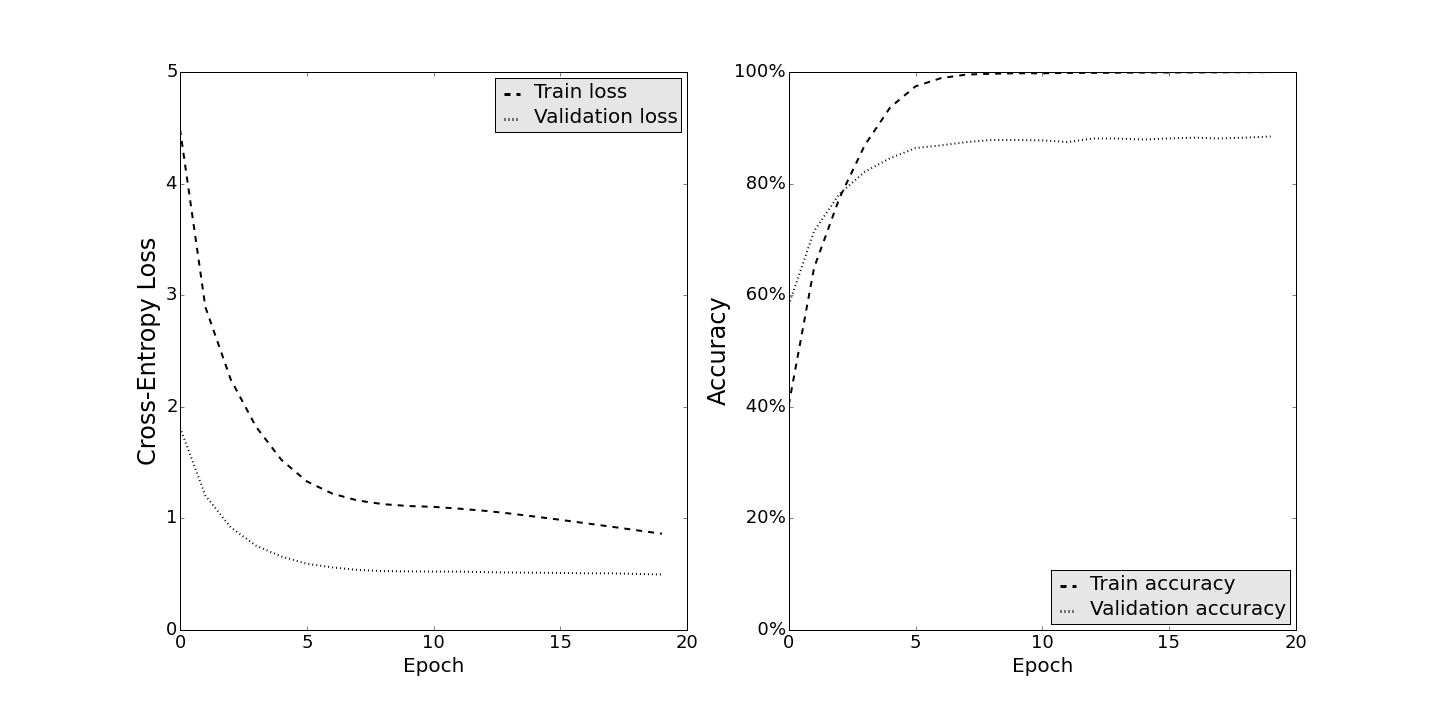
\includegraphics[width=\linewidth]{appendix-bn_triangular_dropout-fc_e20.png}
	\caption{Dropout (0.5) between fully connected layers }
	\label{fig:app_dropout_exp}
\end{figure}


\subsubsection{Maxpooling}
Running a quick experiment (\cref{fig:app_maxp_exp}), where the maxpooling after the first convolutional layer was removed, has shown that the accuracies turn out much worse (see \cref{tab:app_maxp_experiment-results}).
\begin{table}[!h]
	\begin{center}
		\begin{tabularx}{\linewidth}{|X|l|l|}
			\hline \textbf{Experiment} & \textbf{Validation Acc*} & \textbf{Test Acc*}\\ 
			\hline base line, \cref{fig:app_maxp_base} & 81.36\% & 84.30\% \\
			\hline no maxpooling after conv1, \cref{fig:app_maxp_exp} & 73.30\% & 74.27\% \\
			\hline
		\end{tabularx}
	\end{center}
	\caption{Maxpooling experiment results - Not considering imbalance of categories}
	\label{tab:app_maxp_experiment-results}
\end{table}
\begin{figure}[H]
	\includegraphics[width=\linewidth]{{appendix-bn_lr-0.02_e4}.png}
	\caption{Base line for maxpooling experiment }
	\label{fig:app_maxp_base}
\end{figure}

\begin{figure}[H]
	\includegraphics[width=\linewidth]{{appendix-bn_lr-0.02_no-maxpooling1_e4}.png}
	\caption{No maxpooling after conv1 }
	\label{fig:app_maxp_exp}
\end{figure}


\subsubsection{Batch Normalization}
For this experiment, we have used the architectures described in \cref{tab:bn-arch,tab:no-bn-arch} and training was done with a fixed learning rate of 0.005.
Comparing \cref{fig:app_bn_base,fig:app_bn_exp} shows that the network converges extremely fast when using batch normalization but settles around the 83\% accuracy mark, while the non-batch-normalized model keeps improving.
We assume that the learning rate decay was not increasing fast enough, as \citet{Ioffe2015} recommend.
\begin{table}[!h]
	\begin{center}
		\begin{tabularx}{\linewidth}{|X|l|l|}
			\hline \textbf{Experiment} & \textbf{Validation Acc*} & \textbf{Test Acc*}\\ 
			\hline base line, lr 0.005, \cref{fig:app_bn_base} & 83.36\% & 83.62\% \\
			\hline no batch normalization, \cref{fig:app_bn_exp} & 84.03\% & 84.00\% \\
			\hline
		\end{tabularx}
	\end{center}
	\caption{Batch normalization experiment results - Not considering imbalance of categories}
	\label{tab:app_bn_experiment-results}
\end{table}
\begin{figure}[H]
	\includegraphics[width=\linewidth]{{appendix-bn_lr-0.005_e40}.png}
	\caption{Base line for batch normalization experiment}
	\label{fig:app_bn_base}
\end{figure}

\begin{figure}[H]
	\includegraphics[width=\linewidth]{{appendix-no-bn_lr-0.005_e40}.png}
	\caption{No batch normalization }
	\label{fig:app_bn_exp}
\end{figure}


\end{document}
